\documentclass[aspectratio=43, 10pt, utf8, mathserif]{beamer}
%导言区
\usepackage{ctex}
\usepackage{amsmath, amsfonts, amssymb, amsthm}
\usepackage{graphicx}
\usepackage{fontspec}
\usepackage{ulem} %解决下划线换行紊乱
\usepackage{caption} %添加图、表的标题
\usepackage{subfigure}
\usepackage{theorem}
\usepackage[backend=bibtex,sorting=none]{biblatex} %不列出所有作者
%\usepackage[backend=bibtex,sorting=none,maxnames=9,minnames=3]{biblatex} %列出所有作者,具体选择列不列可以由其前的“%”来决定
\addbibresource{ref.bib} %BibTeX数据文件及位置
\setbeamerfont{footnote}{size=\tiny} %设置脚注引用文献的字体大小
%\setbeamertemplate{bibliography item}[text] %设置参考文献图标样式数字标号
\usepackage{appendix} %增加附录
\usepackage{multicol} %分栏
\usepackage{syntonly} %只编译文件是否成功,省时省力
%\syntaxonly %不注释代表只编译是否成功
%\usepackage[marginal]{footmisc} %首页添加脚注无缩进
%\renewcommand{\thefootnote}{} %首页添加脚注无编号
\usepackage{enumerate}
\usepackage{listings} %代码包
\usepackage{xcolor} %代码高亮包
\definecolor{jnucolor}{RGB}{48, 127, 142}
\lstset{
	language=Matlab, %代码语言使用的是matlab
	%frame=shadowbox, %把代码用带有阴影的框圈起来
	%rulesepcolor=\color{red!20!green!20!blue!20}, %代码块边框为淡青色
	keywordstyle=\color{blue}\bfseries, %代码关键字的颜色为蓝色,粗体
	commentstyle=\color{orange}\ttfamily, %设置代码注释的颜色,原字体样式\textit
	backgroundcolor=\color{darkgray!6}, %背景色
	showstringspaces=false, %不显示代码字符串中间的空格标记
	numbers=left, %显示行号
	numberstyle=\tiny, %行号字体
	basicstyle=\ttfamily,
	stringstyle=\ttfamily, %代码字符串的特殊格式
	breaklines=true, %过长的代码自动换行
	extendedchars=false,  %解决代码跨页时,章节标题,页眉等汉字不显示的问题
	escapebegin=\begin{CJK*}{GBK}{hei},escapeend=\end{CJK*} %防止中文报错
	texcl=true,
	morekeywords={classdef,function,global,parfor,persistent,spmd,plot}} %设置更多关键词

%使用的主题样式和主题色
%\usetheme{Antibes}
%\usetheme{Marburg} % TOC tab 
%\usetheme{Berkeley} 
%\usetheme{PaloAlto} 
%\usetheme{Goettingen} 
%\usetheme{Hannover}  % ok2 
%\usetheme{Antibes}  % Tree 
%\usetheme{JuanLesPins}  % ok 3 
%\usetheme{Montpellier} 
%\usetheme{Bergen}   % w/o guide 
%\usetheme{boxes} 
%\usetheme{Bergen} 
%\usetheme{Madrid} 
%\usetheme{Pittsburgh} 
%\usetheme{Rochester} 
\usetheme{Berlin}   % mini guide 
%\usetheme{Ilmenau}   %ok 4 
%\usetheme{Dresden} 
%\usetheme{Darmstadt}   %ok 1 
%\usetheme{Frankfurt} 
%\usetheme{Singapore}  % ok ok 
%\usetheme{Szeged} % ok ok ok 
%\usetheme{Copenhagen} 
%\usetheme{Luebeck} 
%\usetheme{Malmoe} 
%\usetheme{Warsaw} 
%\usecolortheme{beaver} 
%\usecolortheme{albatross} %深蓝色
%\usecolortheme{beetle} %蓝灰色
%\usecolortheme{dove} 
%\usecolortheme{fly} 
%\usecolortheme{seagull} 
%\usecolortheme{crane} 
%\usecolortheme{rose} 
%\usecolortheme{lily}   % inner color 
%\usecolortheme{orchid} % inner color 
%\usecolortheme{whale}  % outer color %深蓝色
%\usecolortheme{seahorse} % outer color    %% ok 浅紫色
%\usecolortheme{sidebartab} %浅紫色
%\usecolortheme{dolphin}  % ok ok
\usecolortheme{jnucolor} %暨大校徽的颜色

\usefonttheme{serif} %已有的字体default professionalfonts serif structurebold structureitalicserif structuresmallcapsserif

% 设置用acrobat打开就会全屏显示
\hypersetup{pdfpagemode=FullScreen}

% 设置logo
\pgfdeclareimage[height=1.3cm]{university-logo}{logo} %需提前将logo文件放到`.tex`文件中。
\logo{\pgfuseimage{university-logo}}

\usepackage{listings}
\usepackage{xcolor} 


\definecolor{mygreen}{rgb}{0,0.6,0}
\definecolor{mygray}{rgb}{0.5,0.5,0.5}
\definecolor{mymauve}{rgb}{0.58,0,0.82}
\lstset{ %
	backgroundcolor=\color{white},   % choose the background color
	basicstyle=\footnotesize\ttfamily,        % size of fonts used for the code
	columns=fullflexible,
	breaklines=true,                 % automatic line breaking only at whitespace
	captionpos=b,                    % sets the caption-position to bottom
	tabsize=4,
	commentstyle=\color{mygreen},    % comment style
	escapeinside={\%*}{*)},          % if you want to add LaTeX within your code
	keywordstyle=\color{blue},       % keyword style
	stringstyle=\color{mymauve}\ttfamily,     % string literal style
	frame=shadowbox,
	rulesepcolor=\color{red!20!green!20!blue!20},
	% identifierstyle=\color{red},
	numbers=left, 
	numberstyle=\tiny,
	% escapeinside=' ',
	xleftmargin=2em,
	xrightmargin=2em, 
	aboveskip=1em
}

\usepackage{tikz}
\usetikzlibrary{positioning, shapes.geometric}
\usetikzlibrary{calc}

\tikzstyle{format}=[rectangle,draw,thin,fill=white]  
%定义语句块的颜色,形状和边
\tikzstyle{test}=[diamond,aspect=2,draw,thin]  
%定义条件块的形状,颜色
\tikzstyle{point}=[coordinate,on grid,]  
\tikzstyle{startstop} = [rectangle, rounded corners,minimum height=0.7cm,text centered, draw=black]
\tikzstyle{io} = [trapezium, trapezium left angle=70, trapezium right angle=110,  minimum height=0.7cm, text centered, draw=black]
\tikzstyle{process} = [rectangle,  minimum height=0.7cm, text centered, draw=black]
\tikzstyle{decision} = [diamond, minimum height=0.7cm, text centered, draw=black]
\tikzstyle{arrow} = [thick,->,>=stealth]
\tikzstyle{every node}=[font=\normalsize]


%-------------开始-------------------
\begin{document}
	
	%每个章节都有小目录
	\AtBeginSection[]
	{
		\begin{frame}
			\frametitle{目录}
			\zihao{4}
			\tableofcontents[currentsection]
			
		\end{frame}
	}
	
	\title{电力系统网源协调平台开发}
	
	\author[余思贤]{\zihao{-3}余思贤\\\ 
		\\ \zihao{-4}
		指导老师:莫维科\\\ 
		\\
		国际能源学院-电气工程及其自动化
		\quad \\ \vspace{0.5cm}  \quad\zihao{6}{ }}
	\institute[ ]
	{
		
	}
	\date{\today}
	%显示封面页
	\begin{frame}
		%\maketitle
		\titlepage
	\end{frame}
	
%		\begin{frame}
%			\frametitle{目录}
%			\begin{multicols}{2}
%				\tableofcontents[hideallsubsections]
%			\end{multicols}
%			%\tableofcontents[hideallsubsections]
%		\end{frame}
	
	\section{背景与研究内容介绍}
	
	
%	\begin{frame}
%		\frametitle{研究背景}
%		\zihao{3}
%		近年来,风力发电、光伏发电等新能源发电技术日益成熟,分布式小规模新能源机组并网比例日益增大。
%		\begin{figure}[H]
%			\centering
%			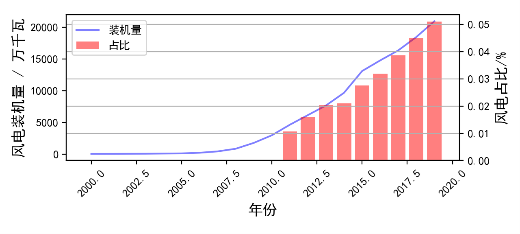
\includegraphics[width=0.5\linewidth]{pic/screenshot005}
%			\caption{近20年来风电装机容量}
%			\label{fig:screenshot005}
%		\end{figure}
%	\end{frame}
%	
%	
%	\begin{frame}
%		\frametitle{新能源机组的并网问题}
%		\zihao{3}
%		
%		\begin{columns}
%			\begin{column}{.5\linewidth}
%				直接并网危害
%				\begin{enumerate}
%					\item 影响电网频率
%					\item 电压波动
%					\item 产生谐波影响
%				\end{enumerate}
%			\end{column}
%			
%			\begin{column}{.5\linewidth}
%				解决办法
%				\begin{enumerate}
%					\item 使用补偿装置
%					\item 使用储能技术
%					\item 网-源-荷协调(辅助服务)
%				\end{enumerate}
%			\end{column}
%		\end{columns}
%	\end{frame}
	
	
	\begin{frame}
		\frametitle{辅助市场前景}
	
	
		
		\begin{columns}
			\begin{column}{.475\linewidth}
					\zihao{3}
				\begin{enumerate}
					\item 新能源大规模发展
					\item 政策利好
				\end{enumerate}
			\end{column}
			\begin{column}{0.05\linewidth}
				\zihao{1}
				\textbf{$ \Rightarrow $}
			\end{column}
			\begin{column}{0.475\linewidth}
					\zihao{3}
				辅助服务能释放出千亿级的蓝海市场,约现在10倍,且随着新能源接入将不断增加。
			\end{column}
		\end{columns}
		
		
	\end{frame}
	
		\begin{frame}
		\frametitle{辅助市场现状}
		\zihao{3}
		\begin{enumerate}
			\item 理解“两项细则” 及辅助服务市场规则需要较高的技术要求
			\item 小电厂没能力、没动力、没资金定制辅助服务分析与控制平台
			\item 新能源场站在考核时亏损巨大
		\end{enumerate}
	\end{frame}
	
	
	\begin{frame}
		\frametitle{毕业设计内容}
		\zihao{3}
		主要针对分布式小装机容量的新能源并网机组,本系统:
		\begin{enumerate}
			\item 提供一套适用于该类机组的网—源协调分析方案
			\item 设计与分析方案相匹配的分析算法
			\item 搭建适用于该类机组的分析平台框架
		\end{enumerate}
	\end{frame}


	\section{系统软件平台}
	
	\begin{frame}
		\frametitle{系统硬件基础}
		\zihao{3}
		\begin{enumerate}
			\item 云服务器$ \times 1$:应用服务器
			\item 本地服务器$ \times 1$:数据库服务器
			\item 开发工作站$ \times 1$:运维
		\end{enumerate}
		
	\end{frame}

		\begin{frame}
		\frametitle{系统整体结构}
		\zihao{3}
		
		\begin{columns}
			\begin{column}{.05\linewidth}
			
			\end{column}
			\begin{column}{.35\linewidth}
				系统结构如下:
				\begin{enumerate}
					\item 前端UI
					\item 控制层
					\item 业务层
					\item 数据层
					\item 数据库
					\item 运行环境
				\end{enumerate}
			\end{column}
			
			\begin{column}{.6\linewidth}
					\begin{figure}[H]
					\centering
					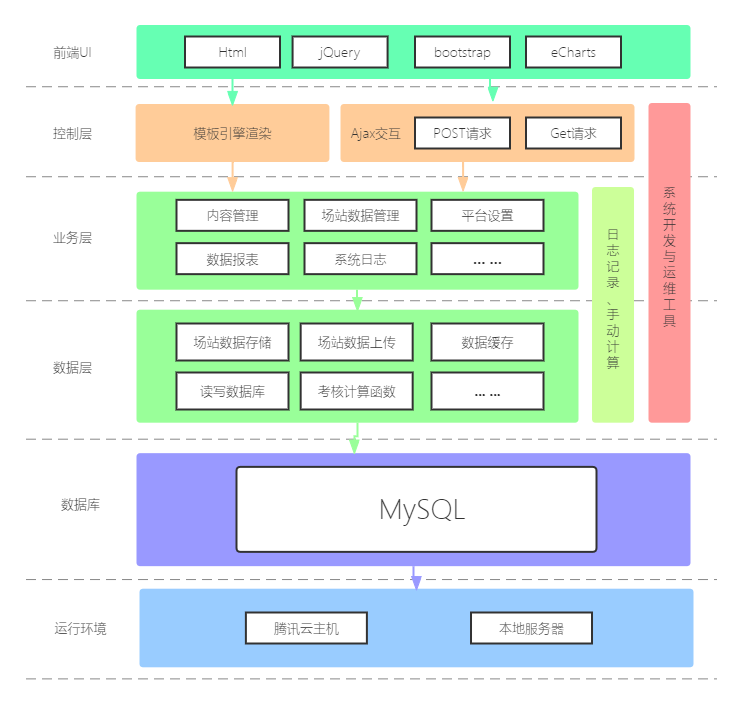
\includegraphics[width=0.93\linewidth]{pic/系统框架结构}
					\caption{系统整体结构图}
					\label{电力系统网源协调控制系统整体结构图}
				\end{figure}
			\end{column}
		\end{columns}
	\end{frame}

	\begin{frame}
		\frametitle{系统运行流程}
		\zihao{3}
		场站侧按照系统要求对场站实际运行数据进行整理和处理,进行数据上传致数据库;数据库以特定格式储存数据后,将数据上传至应用服务器,待计算完成后将储存结果;显示终端则向应用服务器发送POST或GET请求,根据请求显示不同的数据。
		\begin{figure}[H]
			\centering
			
\includegraphics[width=0.95\linewidth]{pic/软件系统示意图}
			\caption{软件系统运行流程}
			\label{软件系统运行流程}
		\end{figure}
	\end{frame}
	
	\section{系统主要算法}
			\begin{frame}
		\frametitle{风光预测考核}
		\zihao{5}
		
		\begin{columns}
			
			\begin{column}{.4\linewidth}
				\zihao{-5}
			\begin{enumerate}
				\item 日预测
				\begin{equation}\label{pre_wind_day}
					\texttt{准确率}=(1-\dfrac{\sqrt{\sum\limits_{i=1}^{n}(P_{Mi}-P_{Pi})^2}}{Cap\sqrt{n}})\nonumber
				\end{equation}
				
				\item 实时预测
				\begin{equation}\label{pre_wind_rt}
					\texttt{准确率}=(1-\dfrac{\sqrt{\sum\limits_{i=1}^{n}(P_{Mi}-P_{Pi,t})^2}}{Cap\sqrt{n}})\nonumber
				\end{equation}
				
			\end{enumerate}
			\end{column}
			
			\begin{column}{.6\linewidth}
			\begin{figure}[H]
				\centering
				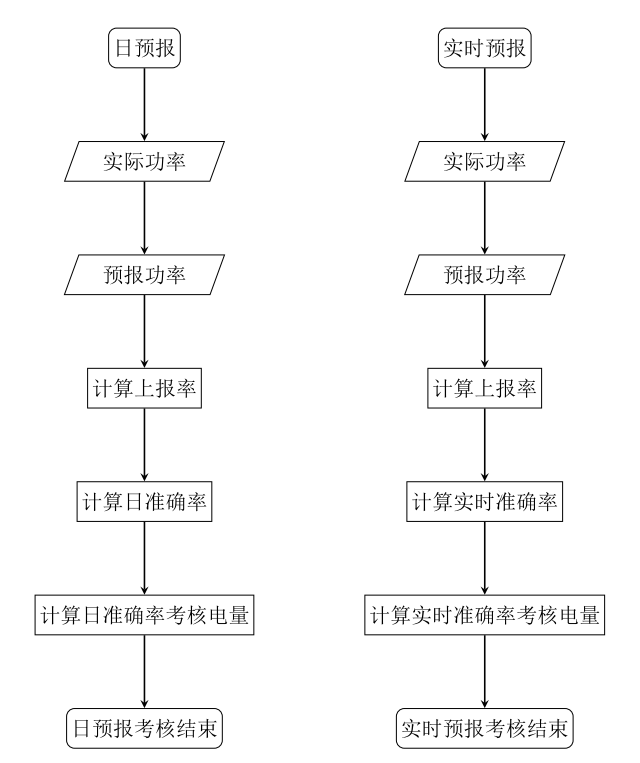
\includegraphics[width=0.75\linewidth]{pic/screenshot028}
				\caption{风光预测计算流程图}
				\label{fig:screenshot028}
			\end{figure}
			
			\end{column}
		\end{columns}
	\end{frame}


	\begin{frame}
		\frametitle{一次调频积分电量考核}
		\zihao{3}
		机组一次调频理论积分电量计算方法:
		\zihao{4}
		\begin{equation}
			\left\{	\begin{aligned}
				 Q_{e}&=\int_{t_{0}}^{t_{1}} \Delta P(\Delta f,t)\mathrm{d}t\\
				\Delta P(\Delta f,t)&=P_{n}\dfrac{\Delta f(t)}{f_{n}}\dfrac{1}{e_{p}}\\
				\Delta f(t)&=|f_{t}-f_{n}|-f_{\texttt{人工死区}}\nonumber
			\end{aligned}\right.
		\end{equation}
	\end{frame}

	\begin{frame}
	\frametitle{一次调频积分电量考核}
	\zihao{3}
	机组一次调频实际积分电量计算方法:
	
	\ \\
	
	\zihao{4}
	\begin{equation}
		\left\{	\begin{aligned}
			Q_{a}&=\int_{t_{0}}^{t_{1}}\Delta P(t) \mathrm{d}t\\
		\Delta P(t)&=P_{a}-P_{0}\nonumber
		\end{aligned}\right.
	\end{equation}
\end{frame}


	\begin{frame}
	\frametitle{一次调频积分电量考核}
	
	\begin{columns}
		\zihao{-3}
		\begin{column}{.4\linewidth}
			\begin{enumerate}
				\item 判断一次调频是否动作
				\item 计算频率差和功率差
				\item 判断是否合格
			\end{enumerate}
		\end{column}
		
		\begin{column}{.6\linewidth}
		\begin{figure}[H]
			\centering
			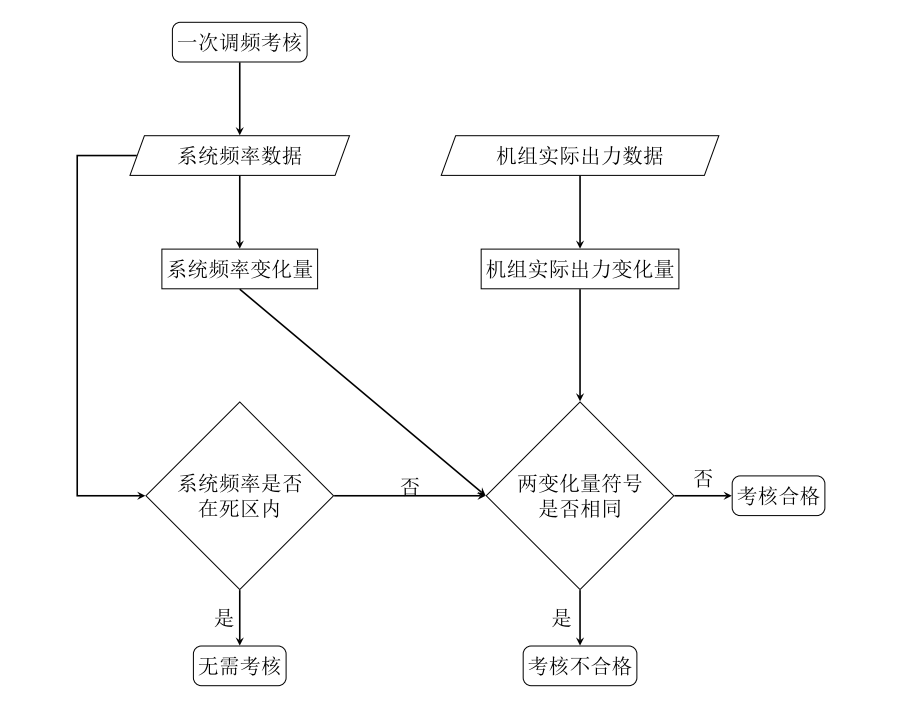
\includegraphics[width=1.05\linewidth]{pic/screenshot030}
			\caption{第一步计算流程图}
			\label{fig:screenshot030}
		\end{figure}
			
		\end{column}
	\end{columns}
\end{frame}



	\begin{frame}
	\frametitle{一次调频积分电量考核}
	
	\begin{columns}
		\zihao{-3}
		\begin{column}{.4\linewidth}
			\begin{enumerate}
				\item 计算实际出力积分电量
				\item 计算理论出力积分电量
				\item 判断二者之比是否在规定值以内
				\item 判断是否合格
			\end{enumerate}
		\end{column}
		
		\begin{column}{.6\linewidth}
		\begin{figure}[H]
			\centering
			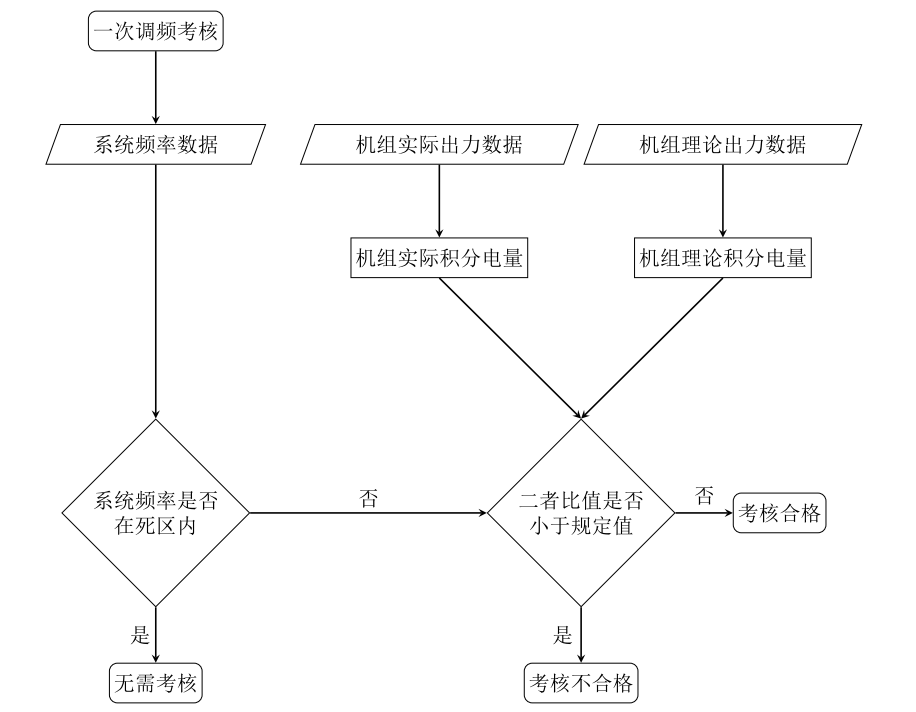
\includegraphics[width=1.03\linewidth]{pic/screenshot031}
			\caption{第二步计算流程图}
			\label{fig:screenshot031}
		\end{figure}
			
		\end{column}
	\end{columns}
\end{frame}



%\begin{frame}
%	\frametitle{前端UI绘图自动缩放}
%	\zihao{3}
%	
%\begin{figure}[H]
%	\centering
%	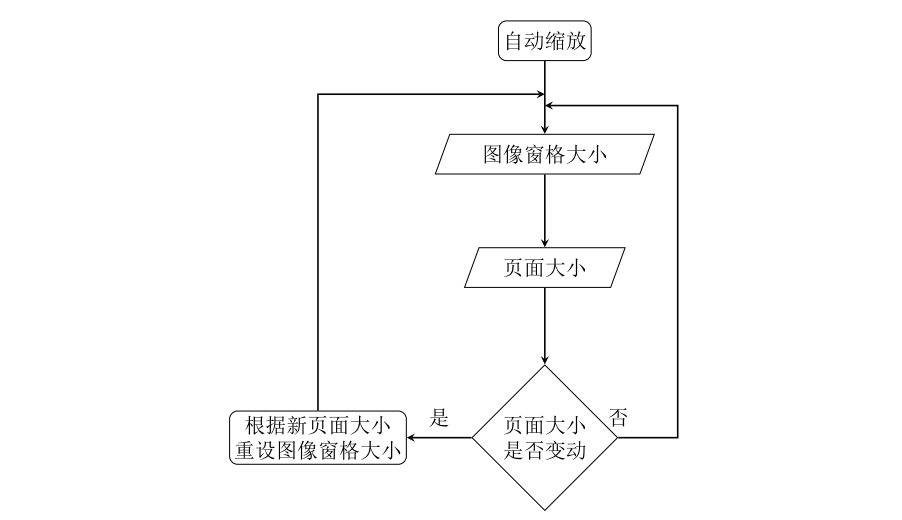
\includegraphics[width=0.7\linewidth]{pic/screenshot032}
%	\caption{自动缩放实现流程图}
%	\label{fig:screenshot032}
%\end{figure}
%\end{frame}
%
%\begin{frame}
%	\frametitle{前端UI绘图自动缩放}
%	\zihao{3}
%	
%	\begin{figure}[H]
%		\centering
%		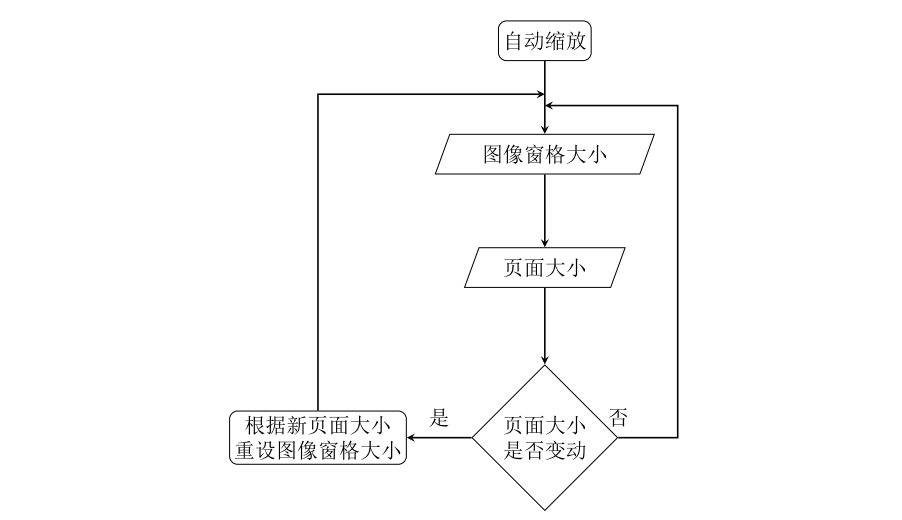
\includegraphics[width=0.7\linewidth]{pic/screenshot032}
%		\caption{自动缩放实现流程图}
%		\label{fig:screenshot032}
%	\end{figure}
%\end{frame}
%
%\begin{frame}
%	\frametitle{前端UI提示框位置修正}
%	\zihao{3}
%	
%\begin{figure}[H]
%	\centering
%	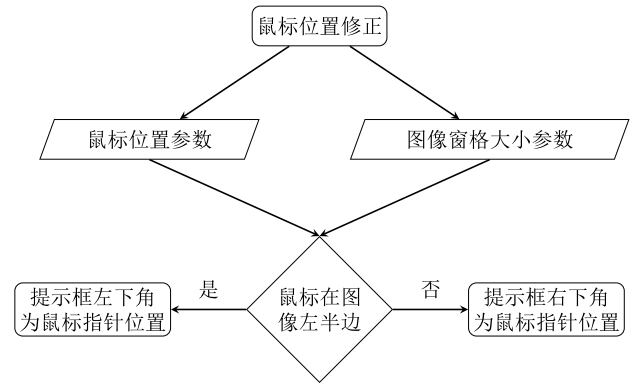
\includegraphics[width=0.6\linewidth]{pic/screenshot033}
%	\caption{提示框位置修正实现流程图}
%	\label{fig:screenshot033}
%\end{figure}
%\end{frame}
%
%\begin{frame}
%	\frametitle{前端UI表格绘制}
%	\zihao{3}
%	
%\begin{figure}[H]
%	\centering
%	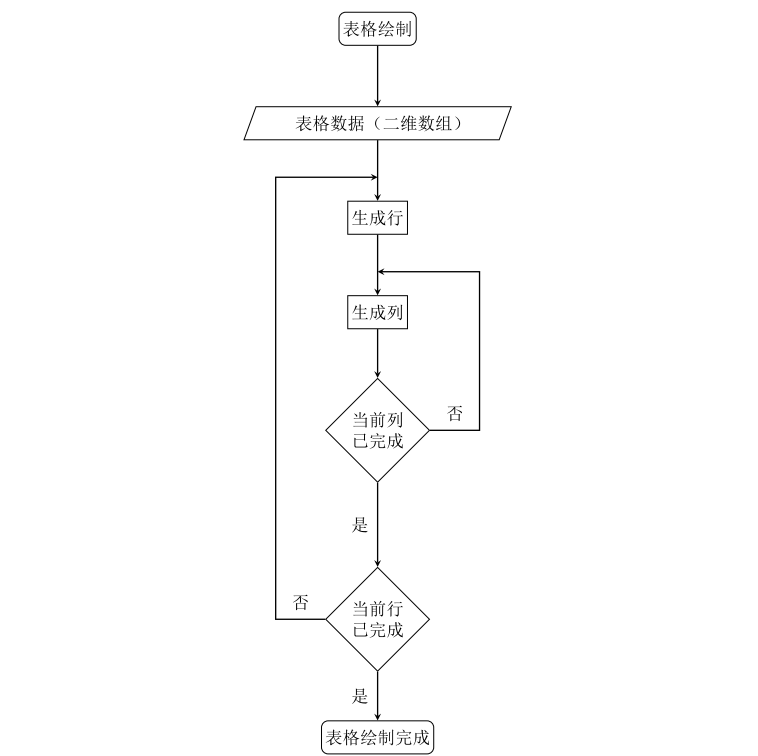
\includegraphics[width=0.4\linewidth]{pic/screenshot034}
%	\caption{表格绘制实现流程图}
%	\label{fig:screenshot034}
%\end{figure}
%\end{frame}

\section{系统平台DEMO演示}

		\begin{frame}
	\frametitle{DEMO演示}
	\zihao{5}
	
	\begin{columns}
		
		\begin{column}{.4\linewidth}
			\zihao{4}
			可以通过如下网址进入系统平台DEMO:http://software\_demo.eew
			
			kmo.cn:8086/
		\end{column}
		
		\begin{column}{.6\linewidth}
			\begin{figure}[H]
				\centering
				
\includegraphics[width=0.8\linewidth]{pic/screenshot035}
				\caption{DEMO演示网址二维码}
				\label{fig:screenshot035}
			\end{figure}
			
		\end{column}
	\end{columns}
\end{frame}



%\begin{frame}
%	\frametitle{DEMO演示}
%	\zihao{4}
%	可以通过如下网址进入系统平台DEMO:http://software\_demo.eewkmo.cn:8086/
%\begin{figure}[H]
%	\centering
%	
\includegraphics[width=0.35\linewidth]{pic/screenshot035}
%	\caption{表格绘制实现流程图}
%	\label{fig:screenshot034}
%\end{figure}
%\end{frame}
\section*{结束}

\begin{frame}
	\zihao{-0}\centering{谢谢各位老师
		
		请老师们批评指正}
\end{frame}

\begin{frame}
	 \zihao{0}\centering{谢谢}
\end{frame}


\end{document}